\newpage

\subsection{Имитационное моделирование}

Необходимо выполнить имитационное моделирование рассматриваемой системы средствами языка GPSS.\par\bigskip

Структура программы:\\
\verb|INITIAL| -- блок задания количественных и временных параметров исходных данных моделируемой системы;\\
\verb|STORAGE| -- блок задания многоканальных узлов системы;\\
\verb|FUNCTION| -- блок задания функции распределения запросов по узлам и времени выполнения запросов в узлах;\\
\verb|GENERATE| -- блок генерации количества задач, циркулирующих в системе;\\
\verb|PCF| -- метка, объединяет набор блоков, описывающих формирование запроса на рабочей станции;\\
\verb|CAN| -- метка, объединяет набор блоков, описывающих обработку эапроса в канале;\\
\verb|SRV| -- метка, объединяет набор блоков, описывающих обработку эапроса в процессоре;\\
\verb|PER| -- метка, объединяет набор блоков, описывающих правило перехода запроса после обработки на диске в канал;\\
\verb|PCD| -- метка, объединяет набор блоков, описывающих дообработку запроса на рабочей станции.\par\bigskip

Текст программы на языке GPSS:
\begin{verbatim}
INITIAL X$STATION_N,19   ; количество рабочих станций
INITIAL X$STATION_TD,190 ; время на дообработку запроса
INITIAL X$STATION_TF,190 ; время на формирование запроса
INITIAL X$CPU_T,20       ; время обработки процессором
INITIAL X$DISK_N,3       ; количество дисков
INITIAL X$DISK_T,20      ; время обработки на диске
;INITIAL X$CANAL_T,5

FLAG1 VARIABLE 0
FLAG2 VARIABLE 1

WORKSTATION_D  STORAGE 19
WORKSTATION_F  STORAGE 19
WORKSTATION_PC STORAGE 19
CPU            STORAGE 1

DISK_N FUNCTION RN1,D2
0.5,1/1,2

EXPON               FUNCTION                RN1,C23
0,0/.1,.104/.2,.222/.3,.355/.4,.510/.5,.69/.6,.915/
.7,1.2/.75,1.37/.8,1.5/.84,1.83/.88,2.12/.9,2.3/
.92,2.52/.94,2.82/.95,2.98/.96,3.2/.97,3.5/.98,3.9/
.995,5.3/.998,6.2/.9995,7/1,8

GENERATE ,,,X$STATION_N
ASSIGN FLAG1,V$FLAG1
ASSIGN FLAG2,V$FLAG2

PCF QUEUE   QSYSTEM
    QUEUE   QREACTION
    ENTER   WORKSTATION_F,1
    ADVANCE X$STATION_TF,FN$EXPON
    LEAVE   WORKSTATION_F,1
    ASSIGN  3,SRV
    TEST E  P$FLAG1,P$FLAG2,CAN
    LEAVE   WORKSTATION_PC,1

;CAN QUEUE   QCANAL
    ;SEIZE   CANAL
    ;DEPART  QCANAL
    ;ADVANCE X$CANAL_T,FN$EXPON
    ;RELEASE CANAL
CAN TRANSFER ,P3

SRV QUEUE    QCPU
    ENTER    CPU,1
    ADVANCE  X$CPU_T,FN$EXPON
    LEAVE    CPU,1
    DEPART   QCPU
    ASSIGN   5,FN$DISK_N
    QUEUE    P5
    SEIZE    P5
    DEPART   P5
    ADVANCE  X$DISK_T,FN$EXPON
    RELEASE  P5
    TRANSFER 0.0, PER,SRV

PER ASSIGN   3,PCD
    TRANSFER ,CAN

PCD DEPART   QREACTION
    ENTER    WORKSTATION_PC,1
    ENTER    WORKSTATION_D,1
    ADVANCE  X$STATION_TD,FN$EXPON
    LEAVE    WORKSTATION_D,1
    DEPART   QSYSTEM
    ASSIGN   FLAG1,1
    TRANSFER ,PCF

    GENERATE  100000
    TERMINATE 1
    START     1
\end{verbatim}

Так как канал в рассматриваемом варианте модели отсутствует, то соответствующие строки закомментированы.\par\bigskip

\newpage

Результаты имитационного моделирования представлены в таблице~\ref{table:imit_result}.

\begin{table}[h]
\caption{Результаты имитационного моделирования}
\label{table:imit_result}
\centering
 \begin{tabular}{c}
 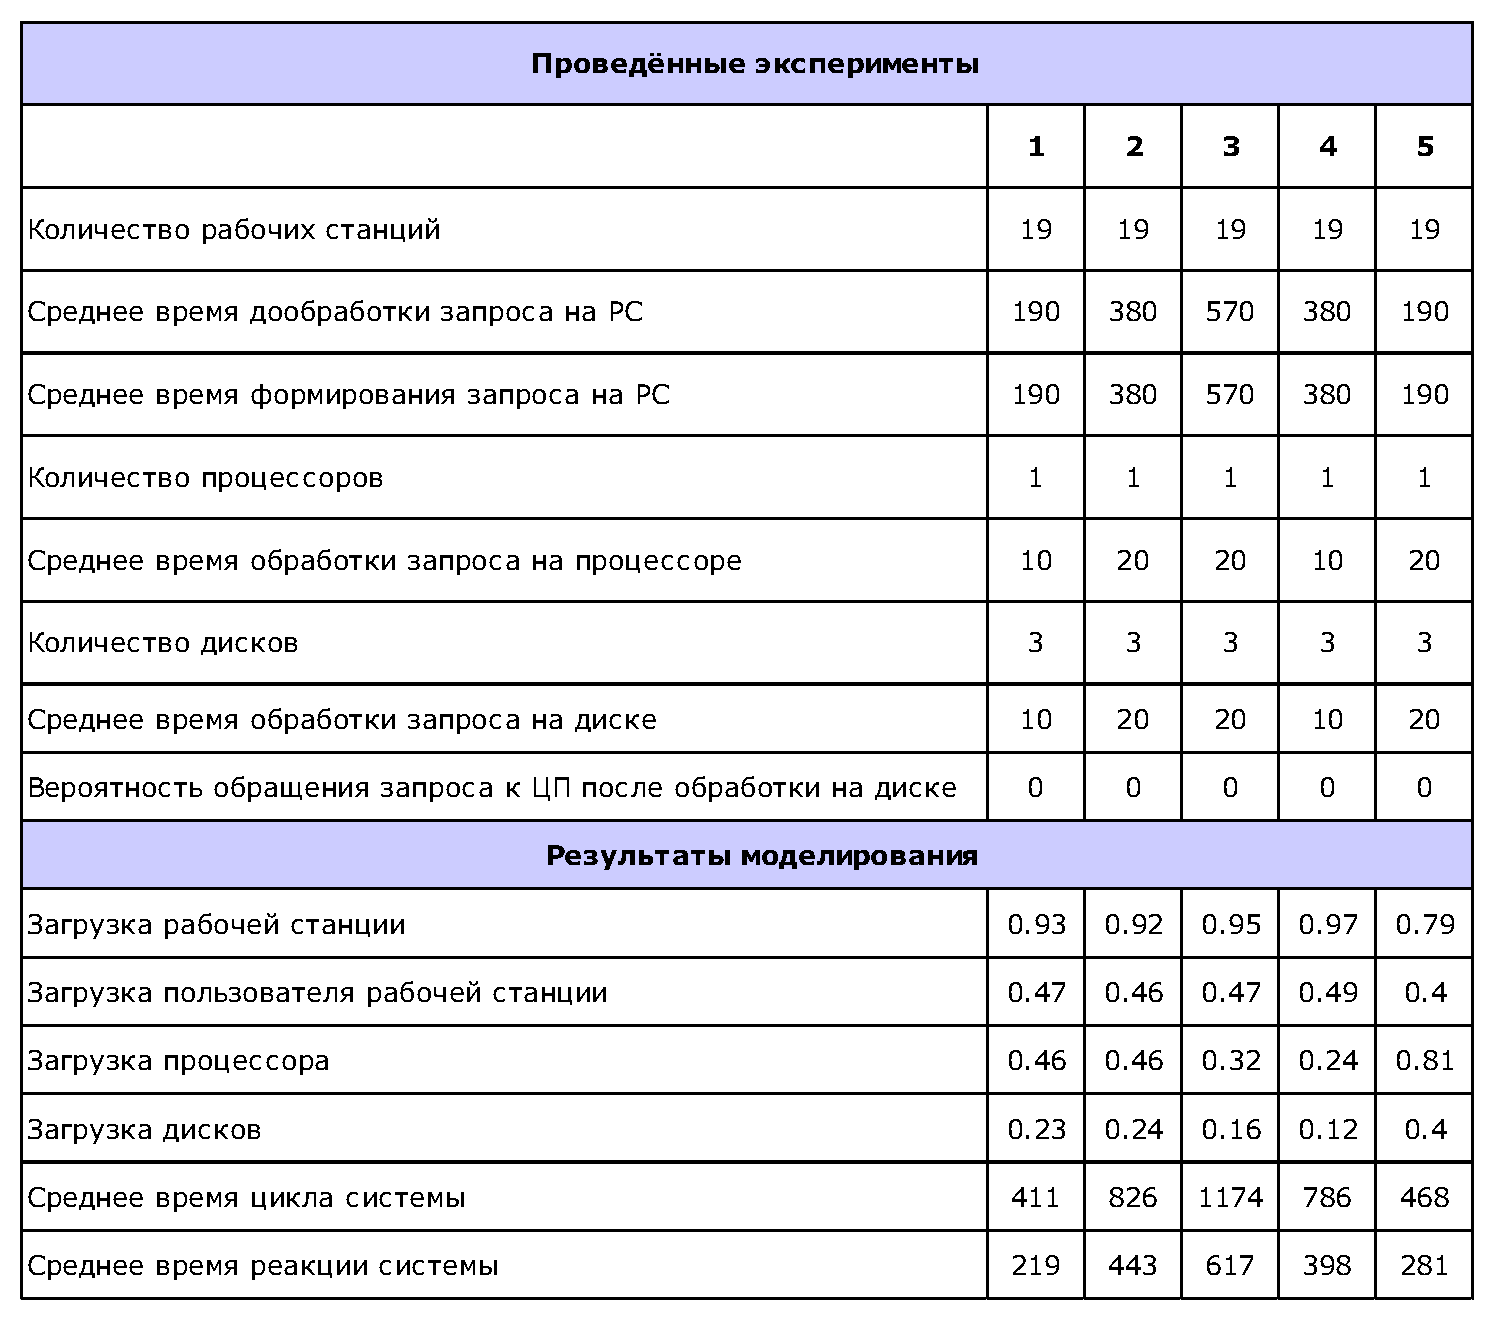
\includegraphics[width=0.7\linewidth]{pics/pic11_1_imit_result.eps}
 \end{tabular}
\end{table}